\documentclass[11pt]{article}
\usepackage{graphicx}
\usepackage[margin=1.5in]{geometry}
\begin{document}

\title{Decentralized Prediction of Social Harm Events}
\author{Dorel Stoian and Zach Spicklemire}

\maketitle
\cleardoublepage

\begin{abstract}
  This paper details our attempt to expand the T-CDASH app to utilize a distributed approach to trust estimation. To accomplish this, a distributed interface was created, various trust nodes were created implementing that interface, and a trust node aggregator was created to consume those trust nodes, and aggregate their results. Using this strategy, we were able to get the advantages of a multi-model approach while distributing the enhanced load of running the multiple trust types over several distributed CPU's.
\end{abstract}

\tableofcontents

\cleardoublepage

\section{Introduction and Problem Statement}

The human interactions in a community involve complex factors and models. Inevitably, friction and harmful events happen. In order to better allocat the resources designed to prevent, stop, or investigate harmful events, different tools have been designed and used. One of these tools is the Trusted Community Data Analytics for Social Harm (T-CDASH), presented in Saurabh Pramond Pandey's thesis ``Trust Estimation of Real-Time Social Harm Events''.This application attempts to predict occurences of social harm events and generate recommendations to prevent them. It is composed of different modules with specific purposes \cite{trust}. 

One of these modules is the trust service, which was designed to analyze the reports of social harm and decide if they will be accepted and passed to the module responsible for predicting future events. Unfortunately, individuals reporting these events may due so incorrectly due to stress and pressure, or may malicously report false information. The concept of the Trust Service tries to mitigate the effects of these false reports of harmful events on the application outcomes \cite[p.~25-44]{trust}.

The implemntation of the Trust Service in the above mentioned application was based on different types of trust models that were progremed to run one at a time. These trust models were employed both to process database entries used to train the machine learning module created to predict events, but also live event reports. Testing these trust models on different sets of data resulted in different levels of accuracy for the predicitons generated by the application \cite[p.~44-45]{trust}.

Analysing the results of the different experiments with trust models raised a question: since one important component of the prediction model is the data that is fed to it, is it possible to increase the application prediction accuracy by feeding into the system data that is more reliable and accurate?

Our project focused on atempting to design a system that will use different types of trust models to analyze the information recieved. The project objectives were both to design these models of trust at the conceptual level and to implement them to run simultaneously, in a distributed environment.

\section{Design Details}

The first decision that had to be made was the overall architecture. The current process was running on a single machine, so it would make sense to have that machine send out work to a number of worker nodes, and then gather the results. We call the worker nodes TrustingNodes and the central node that sends them work and aggregates the results the TrustingNodeAggregator. We considered different ways of distributing the work. The first options considered was that each node would support a different trust model, and each node would recieve all the data. This was very simple, but could be ineffiecent with the communication. Second, we considered having each node implement all the trust types, and having the central node send each a subset of the data. This would be a bit more complicated as we would have to figure out how to partition the data, but it would save on communications. Fianlly, we considered a combination of the two, where we would have multiple clusters of nodes, each cluster would support all the trust types, and work on a part of the data. This could be a best of both worlds. However, we decided to start simple, and try to get the first option working first, and try the others if we got the time. See figure \ref{arch} for the reference.

\begin{figure}
  \centering
  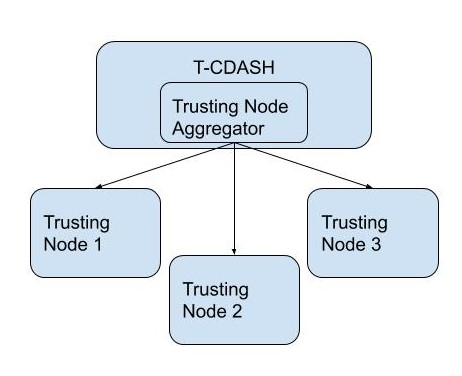
\includegraphics[width=.5\textwidth]{pics/Architecture.jpg}
  \caption{Architecture of Distriubted System}
  \label{arch}
\end{figure}

This architectural model is client-server, the Trust Nodes act as servers, and the Trusting Node Aggregator acts as a client to each of the trust nodes, making calls to them to distribute the work, and consuming their responses.

For our communication model, we decided to have each node act exclusively as a server to the aggregator. The aggregator would initiate all communication and the node would return a response. We considered allowing the aggregator to send over a batch of rows, and receive a batch response to minimize communication overheads, but decided to proceed with the simpler, one row at a time communication first. Each node would return just it's rating (-1 or 1) as a response.

The interaction model for this communication is synchronous, as each trust is communicated to synchronously, with the thread waiting after making the call to the trust node untill the respnose is recieved.

For our secuirty model, we determined that the data records send from the aggregator to the nodes was sensitive, and would have to be encrypted. Since the request data was encrypted, the response data would not be meaningful to intruder, so the response data would not need to be encrypted.

Our for our failure model, the Trusting Nodes can fail by hanging or crashing at any time. The network can also drop packets causing delays in communications (RMI will take care of retrying in the case of dropped packets).

\section{Implementation Details}

First, we had to decide on how the nodes would communicate with each others. The first option was to use Java RMI \cite{rmi}. RMI is bundled with java, very easy to use, and provides some reliablilty built in. We also evaluated using a restful HTTP API. This would require more work on our side to implement but it would allow us to implement TrustingNodes in laguages other than Java. However in the end, we decided we didn't need to use other languages, and decided on RMI.

Since Java RMI does not provide any secrity by default, we decided to implement encryption for our communications. The data sent by the TrustingNodeAggregator to the TrustingNodes would be encrypted. After looking at several algorithms, we decided on AES \cite{aes}. AES uses a very strong algorithm, and is a well supported standard, so it's trustworthy and easy to implement.

\subsection{Aggregator}

The aggregator is the central piece of the system, and so it's performance is critical to the performance of the system as a whole. The Aggregator accepts in it's constructor a list of RMI remote objects representing the remote TrustingNodes. This list can be of any size, so the Aggregator can handle any number of remote nodes cleanly. The most imporatant issue performance wise, is to avoid parts of the processing from waiting needlessly on each other. To accomplish this, we broke each part of the process into runable classes that could be executed in different threads and communciate to each other via concurrent queues. This was broken out as follows

\begin{itemize}
\item A ingester, which will read the data in line by line, and queue it for each of the processors, and the combiner. Once the data is finished, a special ``Done'' message is placed on each queue, so the thread can cleanly exit.
\item A processor for each remote. The processors will recieve the data queued for them by the ingester, make the remote call to the RMI remote server, and put the results onto a queue to be used by the combiner. If the queue runs out before the ``Done'' message is recieved, the thread will sleep for 10ms to allow teh ingester to get some more rows queued.
\item A combiner, which will pull input values from the ingester, then if all the processors have queued a result for that record, will combine their results and decide if it should queue the input record to the final output. If any of the processors have not caught up, it will sleep for 10ms to allow them to catch up, and check again.
\end{itemize}

See figure \ref{agg} for reference.

\begin{figure}
  \centering
  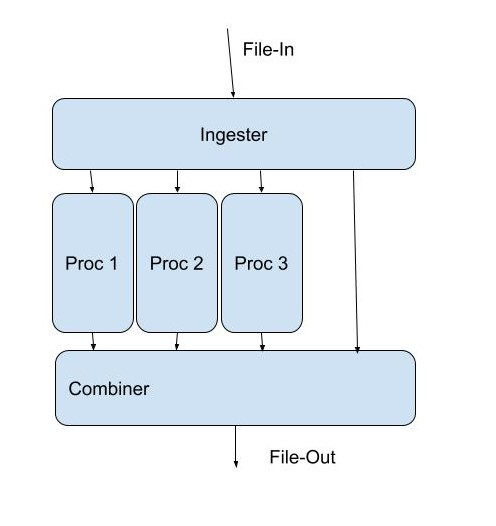
\includegraphics[width=.5\textwidth]{pics/Aggregator.jpg}
  \caption{Threads in the Aggregator}
  \label{agg}
\end{figure}

The Trusting Node Aggregator can process different types of data. Some of them can be publicly accessable, but other can have restricted access. In order to procet the privacy of the data sent to the trsuting nodes for processing, encryption was implemented. The method ``encryptOutGoingMessage'' encrypts the message sent to the node using the AES algorithm and the Cypher class, from the javax.crypto library.

\subsection{Differential Trusting Node}

This node tries to decide if a live report or record should be acepted or not based on the type of event that is being analyzed. In order to achieve this, three classes of events were created:

\begin{itemize}
\item First, events that are considered being such a high probably of being accurate that they are always accepted. Events in this category are traffic stops, directed partols, court ordered property holds and a few others that are usually reported by public authorities and law enforcement personnel. People reporting these types of events have both the professional training and motivation to reliably recogize and report events, and because of that, they are given the highest rate of accuracy.
\item The second class contains reports of events with a higher than average proability of being accurate. The events in this category are accepted at an 85\% rate. Some of the events in this category are traffic accidents, burglaries, kidnappings, robberies, shootings, and a good number of others. These types of events are trusted at a high rate due to the fact that false reporting of such serious events can carry heavy penalties, and as such, they are rarely falsely reported, although it does happen occasionally.
\item Finally, all other events not part of the two above categories are considered of medium accuracy, and are accepted at a 50\% rate.
\end{itemize}

To implement these concepts, two lists of strings were used, one for the 100\% category, and one for the 85\% category. They are initialized in the constructor with the corrisponding values for each category. When the evaluateDataEntry method is invoded for this node, it first decrypts the message received and then extracts the type of event.

The node then checkes each of the above lists to see if the newly acquired type is contained in one of the two lists of strings. If the value matches the content of one of the lists, then the method decides the value to be returned according the the given category, always returning 1 for the 100\% category, and with an 85\% chance of a 1, and a 15\% chance of -1 for the 85\% category.

If the extracted type of event doesn't match the content of either of the two lists, it is assumed to be in the 50\% category. In this case, it will return a 1 or -1 with a 50\% chance of either. The return value, being numeric, and containing no sensitive data, does not need to be encrypted, and is sent directly to the invoker.

\subsection{Exponential Moving Average Trusting Node}

The EMA trusting node keeps an Exponential Moving Average of the probablilty for each Event Type that the node has seen so far. An Exponential Moving Average is a type of Weighted Moving Average. A moving average means instead of keeping all the privious data, only the current average, and the current count are kept. Weighted means that all the events are not treated equally in the average. The formula for calculating the new value of an Exponential Moving Average given a new value \(p_n\), a previous average \(p_{n-1}\), and previous weighted count \(c_{n-1}\) and a scaling factor \(\alpha\) is

\[EMA_n = \frac{WeightedSum_n}{WeightedCount_n} = \frac{p_n + (1-\alpha)p_{n-1}}{1+(1-\alpha)c_{n-1}}\]

This will weight more recent data over older data, so the average will respond strongly to a cluster the same event in a short period of time, but if events are scattered, it will fall off quickly.

\section{Results}

We ran our tests on a sample file containing 54,015 entries, using the Differential Trust Node, the EMA Trust Node, and the Pessimistic Trust Node. Our simulation included both running all nodes at the same time, and also each trust node on it's own, one at a time.

The first thing we noticed is that the time to process the testing data file,while running all three nodes at the same time, and when running each node individually, varried between 14,893 milliseconds and 16,342 milliseconds, with the higher values recorded fro running the nodes individually (for the Differential and EMA Trust Nodes).This gave us an average of 3.6 data entries analyzed per millisecond. See figure \ref{times} for reference.

\begin{figure}
  \centering
  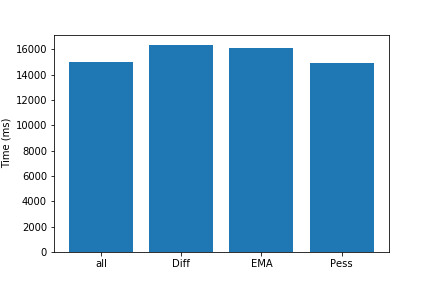
\includegraphics[width=.5\textwidth]{pics/times.png}
  \caption{Total processing time by trusting node}
  \label{times}
\end{figure}

Looking at this data, one conclusiong that can be inferred from it is that if needed, more trust nodes could be added to run in the same timeframe without affecting the overall performance, since adding additional trust nodes does not seem to measurably slow the system down, at least at the scale we have been running at. This easy scalability is probably the biggest advantage of running in a distributed mode, compared to running all the computation in the same node, since more complex and process intensive algrotithms can have their computation distributed accross more CPU's.

Looking to the generated output files, we noticed that the Differential Trust Node had the highest rate of data entries accepted, with an 85\% acceptance rate. The EMA trust node had the lowest rate, with only 0.11\% data entreis being accepted. When we combined all three nodes, the ration of data entries accepted was about 20\%. See figure \ref{outs} for reference.

\begin{figure}
  \centering
  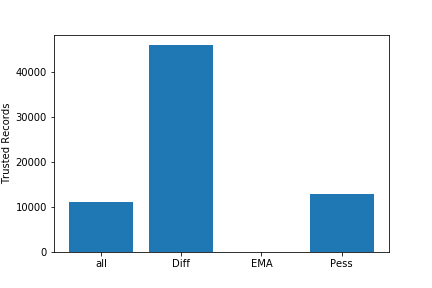
\includegraphics[width=.5\textwidth]{pics/outs.png}
  \caption{Total records trusted by trusting node}
  \label{outs}
\end{figure}

A possible explanation for the obtained results is that the EMA Trust Node is desgined to react strongly to many reports of the same incident type in a short timeframe. It may be more usefule to run it on live reports than on a database or data file where multiple reports of the same event may be reduced to only one entry.

When all three nodes are combined, the influence of one trust node's decision is smaller. The current method used to combine the results from all three nodes is majority vote. Because of this, since one node has a very high acceptance rate, and another has an extreamly low one, the acceptance rate of the third node (in our case, the pessimistic) will have amuch stronger efefct on the final value, and replacing it could have a strong effect on our results.

\section{Conclusion and Future Work}

Overall, we found the trust service concept useful in achieving more accurate predictions. Using multiple trust modes can be beneficial in trying to analyze the data entries and live reports from different perspectives and, in this way, to acchive a higher rate of accuracy in athe data that will be fed to the algorithms used by the predicition module. Java RMI provided a good platform to implement the distributed services used in this projet, and we would recommend it be used in future development.

The current implementation of the distributed trusting nodes could benifit from several extensions. First would be to improve how the trsut node aggregator handles the individual trust nodes. Currently, the aggregator assumes that all nodes will finish their work, and the program will wait indeffinatly if one of the nodes crashes. To improve this, the aggregator could implement a check to periodically see if the trust nodes are still working, and either exclude or restart one that crashes or hangs to allow the process to continue.

Because all the remote nodes are kept in a list, it would be easy to remove one of the remotes from the list, and allow the entire process to keep going. Alternatively, If a node is found to be down, the aggregator could reach out to nodes that it knows about and try to bind another node of the same trust type on another server, and so replace the node that has failed.

A second extesnion of this project could be to desgin the data acquisition part to support more input sources. Currently, the application can read data from a .csv file and writes a new .csv file that contains the accepted data entries. However the T-CDASH app we are trying to integrate with stores and reads from a mysql database. A future extension to allow our module to read from and write to that database would be needed to allow it to integrate with the T-CDASH app.

A third improvement would be to give the users more control in configuring how many and which trust nodes to use. Currently, these are hard coded into the startup of the aggregator, butbetter configuration options or tools could allow the user to easily specify these factors without having to recompile any code. To go even further here, would could move to a three-party architecture, where we have a central registry of trust nodes, which each trust node registers itself with when it comes online. When the aggregator starts it's run, it could reach out to the registry to see what trust nodes and models are available, and potentially automatically choose which ones it binds do based on a set of requirements that changes based on the needs for that run (for example, we have seen that the EMA trust node may perform better for live data than for pre-processed data sets).

Another improvement that can be researched and developed would be to design more sophisticated trust models. Combined with the above improvement to allow the user or the system to choose which trust models to use based on the data and the needs at the time, this could dramatically improve the accuracy of the trust reports, by tailoring the models used to the type of data being processed by the system instead of using a one-size-fits-all approach.

The algorithm for combining the results sent in by the trusting nodes can also be improved. Currently, the algorithm is the very simple majority vote, where each nodes sends a 1 or -1, and their cumlative value is calculated, and is trusted if it's greater than zero. This could be improved in a number of ways, but one simple one would be to weight each trust model by the accuracy it generates when run on it's own, so more accurate models are counted more highly than less accurate ones when combining the results.

Finally, The current communication model for distributing the work is somewhat ineffiecent. Currenlty, each trust node recieves all the data for every record. This could be improved if different nodes were instead responsible for running multiple trust algorithms on different sections of the data. This would allow a specific data record to be sent once instead of once per node. A naive implementation of this could have negative effects on the scalablitliy, but there is likely a good middle ground that exists between every node running one trust type and needed every record, and every node running every trust type and needing only a small section of the data. One such comprimise could be to perform some tracing on each trust algorithm to come up with a loose heuristic on how much CPU and Memory it needs, then groups of trust types could be grouped to run on the same server to make optimal use of the server's resources. We could call a collection of these groupings that contained one of every trust type a Trust Group, and have many Trust Group's running on different servers, such that each Trust Group was working on just one section of the total data. A strategy like this should allow us to make optimal use of our servers resources, and minimize communication overheads.

\cleardoublepage

\addcontentsline{toc}{section}{Critique}
\section*{Critique}

The key concept in the Differential Trusting Node is defining the different categoies of events, and assigning different probability levels for each category. The problem with this approach is how to determine what events should be a part of which category. Some events can look like an easy match for a certain category, but others may require a deeper analysis, and there may be dissagreement, even ammong subject matter experts over which event types belong in what category.

The predition module that uses machine learning to train itself and generate preditions depends significantly onthe data that it is feed. If false data entries or reports are admitted, and valid inputs are discarded at a significant rate, the prediction accuracy will suffer, even if the prediction algorithm is sound.

The Differential Trusting Node has a category of events where all events are accepted, and another category that discards events at a very high rate. Looking at these two extreme categories, the improtance of the event categorization becomes clear. We can easily imagine the impact if an unreliable event type is miscategorized as a sure event, or a sure event is miscategorized as a low probablilty one.

With regards to the EMA Trusting Node, it wound up rejecting the vast majority of the data coming in. The algorithm has a value alpha that could be tuned, and possibly make more accurate predictions of trust. We may also have been using data that was not a very good fit for the EMA algorithm, since we didn't have any live reports, we did not see many close grouping of the same type of report.

For the Trusting Node Aggregator, as mentioned in the Conclusion, one thing that can be improved would be to implemnt a greater quality of serice mechanism to prevent the aggregator from hanging if one of the trusting nodes hangs or crashes. As it is the central piece of our application, any additional error checking and error recovery functionality that we could add to it would pay off greatly.

Overall, we did not get as far as we would have liked to in integrating our distributed trust system in to the T-CDASH application. We underestimated how much effort would be needed to get from the point where we had all completed our individual portions to getting it combined into one application, and then to get it integrated into the T-CDASH application. In retrospect, it would have helped if we had worked more closely together earlier in the project timeline to make sure we were working through any issues in our code earlier in the process, instead of finding the issues near the end, when they are more costly to fix. But despite the issue that we encontered along the way, we believe the underlying architecture of our system is solid, and a good base to continue work towards a distributed trusting system for T-CDASH.

\cleardoublepage
\addcontentsline{toc}{section}{References}
\begin{thebibliography}{9}
\bibitem{trust}
  Saurabh Pramod Pandey
  \textit{TRUST ESTIMATION OF REAL-TIME SOCIAL HARM EVENTS}
  IUPUI Department of Computer Science, August 2019

\bibitem{rmi}
  \textit{Java Remote Method Invocation - Distributed Computing for Java}
  https://www.oracle.com/technetwork/java/javase/tech/index-jsp-138781.html

\bibitem{aes}
  Daemen, Joan; Rijmen, Vincent
  \textit{AES Proposal: Rijndael}
  National Institiute of Standards and Technology, March 9, 2003

\bibitem{book}
  Coulouris, George; Dollimore, Jean; Kindberg, Tim; Blair, Gordon;
  \textit{Distributed Systems. Concepts and Design}
  Fifth Edition; Pearson Education Inc, 2012

\end{thebibliography}

\end{document}